\subsection{OGR Converter Plugin}

% when the revision of a section has been finalized, 
% comment out the following line:
% \updatedisclaimer

The OGR layer converter plugin allows to convert vector data from one OGR-supported 
vector format to another OGR-supported vector format. It is very simple to handle and 
provides functionalities as shown in Figure \ref{fig:ogrconverter_dialog}. The 
supported formats can vary according to the installed GDAL/OGR package.

\begin{itemize}
\item \textbf{Source Format/Datset/Layer}: Enter OGR format and path to the vector file to be converted
\item \textbf{Target Format/Datset/Layer}: Enter OGR format and path to the vector output file
\end{itemize}

\begin{figure}[ht]
   \begin{center}
   \caption{OGR Layer Converter Plugin \nixcaption}\label{fig:ogrconverter_dialog}\smallskip
   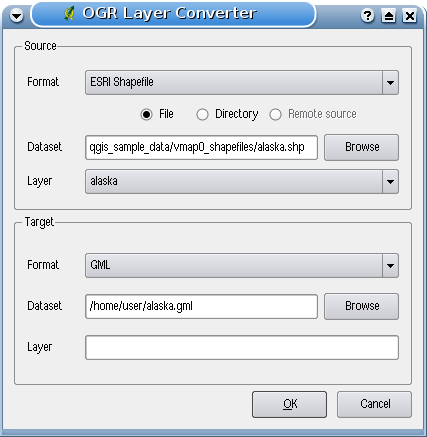
\includegraphics[clip=true, width=9cm]{ogrconverter_dialog}
\end{center}  
\end{figure}

\begin{enumerate}
  \item Start QGIS, load the OGR converter plugin in the Plugin Manager (see Section 
  \ref{sec:load_core_plugin}) and click on the \toolbtntwo{ogr_converter}{OGR Layer Converter} 
  icon which appears in the QGIS toolbar menu. The OGR Layer Converter plugin dialog appears as shown in Figure \ref{fig:ogrconverter_dialog}.
  \item Select the OGR-supported format \selectstring{ESRI Shapefile}{\ldots} and the path to the vector input file \filename{alaska.shp} in the Source area.
  \item Select the OGR-supported format \selectstring{GML}{\ldots} and define a path and the vector output filename \filename{alaska.gml} in the Target area.
  \item Click \button{Ok}.
\end{enumerate}

\newpage



